% siminos/CLE/CLEsols.tex
% $Author$ $Date$

\subsection{\label{s:CLEsols} An example: solutions of \cLe}

In the case of {\cLe}  the origin \EQV{0} is an \eqv\ of
\refeq{eq:CLe} for any value of the parameters. As shown in
\refref{FowlerCLE82} it is stable for $0<\RerCLor<\rho_{1c}$
and unstable for $\rho_{1c}<\RerCLor$, where
\beq
	\rho_{1c} = 1 + \frac{(e+\ImrCLor)(e-\sigma \ImrCLor)}{(\sigma+1)^2}\,.
\eeq
At bifurcation a pair of eigenvalues crosses the imaginary
axis with imaginary part:
\beq
	\omega_c = \frac{\sigma (e + \ImrCLor)}{\sigma+1}\,.
	\label{eq:omegaCLE}
\eeq
and a \emph{relative equilibrium} \REQV{}{1} is born. For
$e+\ImrCLor=0$ the relative equilibrium degenerates to an
\SOn{2}-orbit of \eqva\rf{FowlerCLE82}, since $\omega_c =0$.
Ning and Haken\rf{NingHakenCLE90} and Zeghlache and
Mandel\rf{ZeMa85} use equations isomorphic to \cLe\ with
$e+\ImrCLor=0$ in their studies of detuned ring lasers. From
a symmetry perspective existence of a \reqv\ in a system with
\SOn{2} symmetry is the generic situation, so here we will
stick to the choice $\ImrCLor=0$ and $e \neq 0$ of Bakasov
and Abraham\rf{BakasovAbraham93}.

As $\RerCLor$ is increased,  a secondary bifurcation from
\REQV{}{1} is expected, according to Krupa's
theorem\rf{Krupa90}, to result in \emph{relative periodic
orbits} that satisfy
\beq
	\Rot{\theta_p}x(t+T_p)=x(t)\,.
\eeq
A {\rpo} of {\cLe} is shown in \reffig{fig:CLE}. Its repeats
trace out ergodically a torus, so in a system with a
$1$-dimensional continuous symmetry the organizational blocks
of a strange attractor are circles (\reqva) instead of points
(\eqva), and partially hyperbolic tori (\rpo s) instead of
closed loops (\po s). To understand the geometry of the
system one can choose to look at tori or realize that along
the direction of rotations a tori does not change and pursue
symmetry reduction.

\PublicPrivate{}{
The implications  of this fact are illustrated in
\reffig{fig:CLE}, where we project trajectories in
$(x_1,x_2,z)$ axes, where $x=x_1+ i\, x_2\,,\ y=y_1+i\, x_2$
with $x_i,\,y_i\in\Rls{}$. A generic trajectory slowly `drifts'
along the direction of rotations while tracing a Lorenz-butterfly
like attractor.

 \refFig{fig:CLE} illustrates the need
 to project dynamics on \reducedsp: Dynamics is organized by
 the interplay of the stable and unstable manifolds of \eqv\
 \EQV{0} and \reqv\ \REQV{}{1} but the dynamics along the
 direction of rotation blur the picture and the notion of
 recurrence becomes relative. We will present various
 approaches to orbit space reduction in the following.
    }

 %
%%%%%%%%%%%%%%%%%%%%%%%%%%%%%%%%%%%%%%%%%%%%%%%%%%%%%%%%%%%%
\begin{figure}[ht]
\begin{center}
  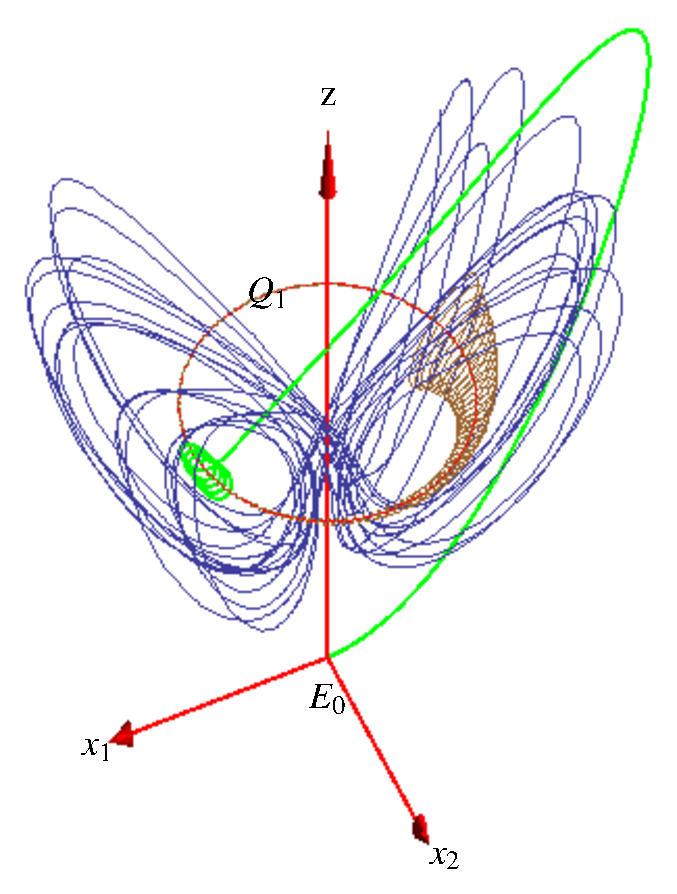
\includegraphics[height=0.25\textheight]{../figs/CLE}
\end{center}
\caption[Complex Lorenz flow phase space]
{ \Statesp\ portrait of \cLe\ dynamics for $e=1/10,\,
\ImrCLor=0$. Plotted are \reqv\ \REQV{}{1} (red), its unstable
manifold (brown), \eqv\ \EQV{0}, a representative of its
unstable manifold (green), 3 repetitions of \rpo\
``01''(magenta) and a generic orbit (blue).}
\label{fig:CLE}
\end{figure}
%%%%%%%%%%%%%%%%%%%%%%%%%%%%%%%%%%%%%%%%%%%%%%%%%%%%%%%%%%%%
%
\marginpar{Split: Fig1: reqb, generic trajectory, rpo. Fig2: reqb, unstable manifolds}

To find the location of the \reqv\ it is convenient to work
on polar coordinates defined by $x=r_1 e^{i \phi_1},\,y=r_2
e^{i \phi_2}$. Equations \refeq{eq:CLe} take the form
    %PC: Rebecca and I rederived these: they check.
\beq
\begin{split}
	\dot{r}_1 &=-\sigma (r_1 - r_2\cos\phi) \cont
	\dot{r}_2 &=-r_2 + r_1(\RerCLor -z)(\cos\phi-\ImrCLor\sin\phi) \cont
	\dot{z} &=  -b z+r_1 r_2\cos\phi \cont	
	\dot{\phi} &=-e-\frac{\sigma r_2 \sin\phi}{r_1}
             -\frac{r_1(\RerCLor-z) (\ImrCLor\cos\phi+\sin\phi) }{r_2}\,,
	\label{eq:CLePolar}
\end{split}
\eeq
where $\phi=\phi_1-\phi_2$ and the evolution equations for
$\phi_1,\phi_2$ are given by
\beq
\begin{split}
	\dot{\phi}_1 &=-\frac{\sigma r_2 \sin\phi}{r_1}\cont
	\dot{\phi_2} &= e +\frac{r_1\left(
         (\RerCLor -z)\sin\phi+\ImrCLor\cos\phi
                                \right)}{r_2}\,.
	\label{eq:CLeAngl}
\end{split}
\eeq

For simplicity we now turn to the ``laser case''
$e\neq0,\;\ImrCLor=0$. The condition for a \reqv\ is that all
time derivatives in \refeq{eq:CLePolar}, while
$\dot{\phi}_1=\dot{\phi}_2\neq 0$. If
$\dot{\phi}_1=\dot{\phi}_2=0$ we would have (a group orbit
of) equilibria. We get
\beq
\begin{split}
	z^{(1)} &= \frac{-e^2+(\RerCLor -1)(\sigma +1)^2}{(\sigma +1)^2}\cont
	r_1^{(1)} &= \sqrt{b z^{(1)}}\cont
	r_2^{(1)} &= \sqrt{b \left(e^2+(\sigma +1)^2\right)z^{(1)}}\cont
	\phi^{(1)} &= -\cos ^{-1}\left(\frac{\sigma +1}{\sqrt{e^2+(\sigma +1)^2}}\right)\,.
\end{split}
\eeq
Substituting in \refeq{eq:CLeAngl} we get
$\dot{\phi}_1=\dot{\phi}_2=e \sigma/(1 + \sigma)\neq 0$ for
$e\neq0$ and thus we have indeed a \reqv, not a group orbit
of \eqva.

Calculation  in polar coordinates $r_1,r_2,\phi,z$ of
stability eigenvalues for \REQV{}{1} for the set of
parameters we use here yields a weakly unstable spiral-out
\eqv\
\beq
	\eigRe[1]\pm i\eigIm[1]= 0.0938\pm 10.1945i,\,
    \eigExp[3]=-11.0009,\, \eigExp[4]= -13.8534\,.
	\label{eq:CLeREQBstab}
\eeq
In \ref{s:StabReq} we show how to calculate stability of
\reqva\ in \emph{equivariant} variables without change of
coordinates to polar or any other set of symmetry invariant
variables.
